\documentclass{article}
\usepackage[utf8]{inputenc}
\usepackage{hyperref}
\hypersetup{
    colorlinks=true,
    linkcolor=blue,
    filecolor=magenta,      
    urlcolor=cyan,
    pdftitle={Overleaf Example},
    pdfpagemode=FullScreen,
    }
\usepackage{tcolorbox}
\tcbuselibrary{theorems}

\usepackage{geometry}
 \geometry{
 a4paper,
 total={170mm,257mm},
 left=20mm,
 top=20mm,
 }
 \usepackage{graphicx}
 \usepackage{titling}

\title{Brain Cancer Segmentation}
\author{Davide Belcastro - Lucian Dorin Crainic}
\date{}
\usepackage{caption}
\usepackage{cite}
\usepackage{float}
\usepackage{multirow}
\usepackage{caption} 

\usepackage{wrapfig}

\usepackage{fancyhdr}
\fancypagestyle{plain}{%  the preset of fancyhdr 
    \fancyhf{} % clear all header and footer fields
    \fancyfoot[L]{\thedate}
    \fancyhead[L]{AI Lab: Computer Vision and NLP A.A 2022/2023}
    \fancyhead[R]{\theauthor}
}
\makeatletter
\def\@maketitle{%
  \newpage
  \null
  \vskip 1em%
  \begin{center}%
  \let \footnote \thanks
    {\LARGE \@title \par}%
    \vskip 1em%
    %{\large \@date}%
  \end{center}%
  \par
  \vskip 1em}
\makeatother

\begin{document}

\newtcolorbox{my theorem}[1]{
colback=black!5,colframe=black!55!black!80,fonttitle=\bfseries, title={#1}}

\newtcolorbox{conlusione}[1]{
colback=purple!5,colframe=purple!55!black!80,fonttitle=\bfseries, title={#1}}
\maketitle

\section{Introduzione}
L'applicazione creata ha come tema principale l'analisi di immagini mediche. Nello specifico,
vengono analizzate immagini di risonanze magnetiche (MRI) al cervello di pazienti. L'applicazione 
si suddivide in 2 parti principali, Segmentazione del tumore e Interfaccia grafica (GUI).

\section{Dataset utilizzati}
Per svolgere l'intero programma sono stati utilizzati 2 dataset differenti
\begin{itemize}
    \item Dataset formato .mat scaricato su kaggle. Il dataset contiene 3064 RMI T1 con mezzo di contrasto svolte a 233 pazienti con 3 tipi di tumori differenti:  meningioma (708), 
    glioma (1426), e pituitary tumor (930).
    Il dataset è suddiviso in 4 directory contenenti 766 file ciascuna.
    Ogni file è in formato matlab(.mat) e contiene le seguenti informazioni
    \begin{itemize}
        \item cjdata.label: 1 for meningioma, 2 for glioma, 3 for pituitary tumor
        \item cjdata.PID: patient ID
        \item cjdata.image: image data
        \item cjdata.tumorBorder
        \item cjdata.tumorMask: a binary image with 1s indicating tumor region
    \end{itemize}

    \item Il primo set di dati è stato scaricato da Kaggle, scaricalo qui. Questo contiene 3264 
    files così divisi, ci sono due directory: "Testing" e "Training", ogni directory contiene 
    altre 4 directory: glioma, pituitary, meningioma, no-tumor. Il formato delle immagini è ".jpg".
\end{itemize}

\section{Segmentazione del tumore}
La segmentazione del tumore è un task molto complesso in quanto le immagini mediche possono avere intensità di luce differenti e riconoscere il contorno di un area anomala all'interno del tessuto cerebrale non sempre risulta essere banale.
Inoltre acquisire un dataset non è semplice per ragioni di privacy sui pazienti.
Per raggiungere l'obiettivo, abbiamo suddiviso il problema in tre principali parti
\begin{itemize}
    \item Skull Stripping
    \item Estrazione del colore medio del tumore
    \item Segmentazione
\end{itemize}
\subsection{Skull Stripping}
Per Skull Stripping si intende l'estrazione del tessuto cerebrale da una MRI andando a eliminare i bordi che possono influenzare la "tumor detection".

\begin{my theorem}{Algortimo}
    Il processo di skull stripping viene fatto andando a calcolare l'intensità del pixel presente con maggior frequenza considerando un range,in un immagine in scala di grigi, tra 20 e 190(non vengono considerati i pixel vicini al nero e vicini al bianco).
    Viene applicato un filtro di Canny per delimitare i contorni nel range che va da -10 a +10 rispetto all'intensità del pixel trovato precedentemente.
    Si cerca di trovare il contorno che più di tutti ha la forma di un cervello andando a prendere solo il tessuto cerebrale(di colore grigio) estrapolando il contorno più esterno.
    L'immagine ritornata non contiene altre parti del corpo che,avendo intensità di luce diverse rispetto al tessuto cerebrale,possono ostacolare il riconoscimento di un tumore, in quanto queste parti potrebbero essere proprio scambiate per tumori.
    L'obiettivo è quello di avere un immagine con solo il cervello,in modo che, qualsiasi differenza netta di intensità possa essere, con molta probabilità, il segmento di un tumore.
\end{my theorem}

\subsubsection{Testing}
% Per valutare l'accuratezza del programma sono stati effettuati dei test sull'intero dataset formato .mat
% Per capire se l'estrazione del contenuto del cervello è avvenuta correttamente,il programma inizialmente calcola l'area del contorno più esterno (tessuto cerebrale + bordo),effettua lo skull stripping e,sul contorno che viene ritornato, calcola l'area e la circolarità.
% Se l'area è troppo piccola rispetto all'area più esterna, o se il contorno è poco circolare, con buona probabilità il processo di skull stripping non ha funzionato correttamente, in caso contrario assumiamo che il processo abbia funzionato correttamente.
% E' presente un caso medio in cui con buona probabilità il processo ha estratto il tessuto cerebrale ma non è riuscito a levare interamente il bordo.
% Illustro un grafico che mostra i risultati del test.

% \begin{figure}[H]
%     \centering
%     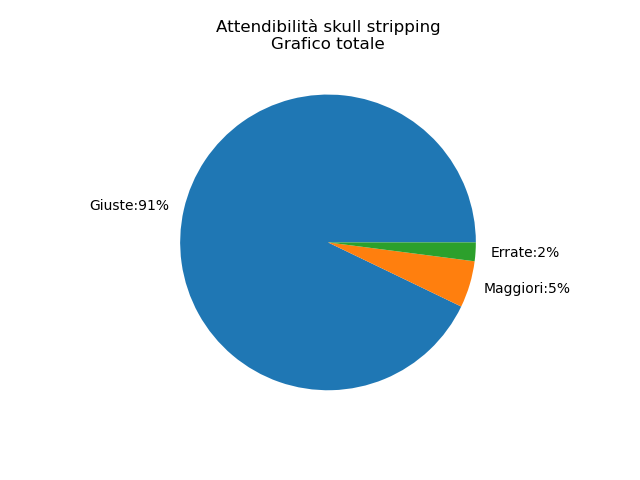
\includegraphics[width=10cm]{images/ss.png}
% \end{figure}

\begin{wrapfigure}{r}{8.5cm}
    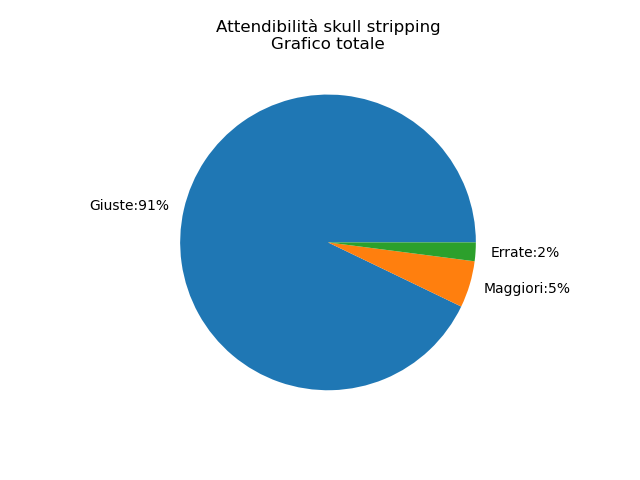
\includegraphics[width=8.5cm]{images/ss.png}
\end{wrapfigure}

Per valutare l'accuratezza del programma sono stati effettuati dei test sull'intero dataset formato .mat
Per capire se l'estrazione del contenuto del cervello è avvenuta correttamente,il programma inizialmente calcola l'area del contorno più esterno (tessuto cerebrale + bordo),effettua lo skull stripping e,sul contorno che viene ritornato, calcola l'area e la circolarità.
Se l'area è troppo piccola rispetto all'area più esterna, o se il contorno è poco circolare, con buona probabilità il processo di skull stripping non ha funzionato correttamente, in caso contrario assumiamo che il processo abbia funzionato correttamente.
E' presente un caso medio in cui con buona probabilità il processo ha estratto il tessuto cerebrale ma non è riuscito a levare interamente il bordo.
Illustro un grafico che mostra i risultati del test.

\hfill \break

\subsection{Estrazione del colore medio del tumore}
In questa fase l'obiettivo è quello di analizzare l'immagine che contiene solo il tessuto cerebrale senza bordi e trovare il colore medio del tumore(qualora sia presente).

\begin{my theorem}{Algoritmo}
    Viene calcolato il colore medio del cervello andando a prendere l'intensità del pixel presente con maggiore frequenza all'interno dell'immagine con solo il tessuto cerebrale.
    A questo punto vengono analizzati tutti i contorni che,oltre a rispettare alcune caratteristiche come la circolarità e l'area, hanno un colore medio distante rispetto al colore medio del cervello.
    Differenza tra colore medio del cervello e colore medio del contorno,uniti ad area e circolarità sono le tre proprietà che caratterizzano e distinguno ogni contorno trovato,il contorno che rispetta maggiormente queste proprietà viene scelto come possibile tumore, e viene restituito il suo colore medio.
    Il colore di questo contorno può non essere del tutto preciso e,come vedremo nel prossimo step, è soltanto un ulteriore parametro che viene utilizzato per confrontarlo con il colore medio dei contorni che vengono analizzati successivamente con maggiore precisione.
\end{my theorem}

\subsubsection{Testing}

\begin{wrapfigure}{r}{8.5cm}
    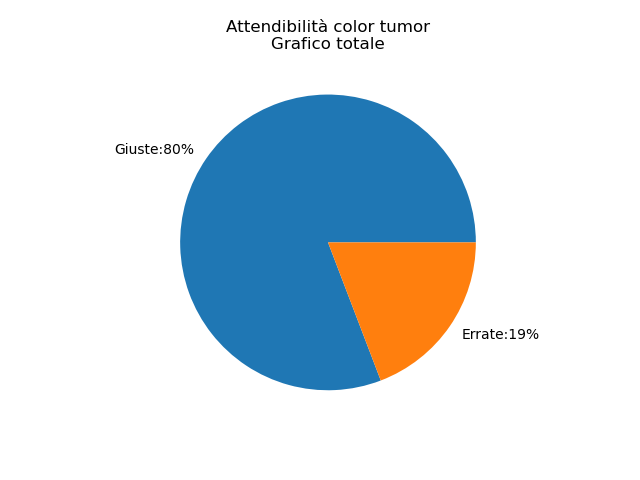
\includegraphics[width=8.5cm]{images/ct.png}
\end{wrapfigure}

In questa fase, per valutare la correttezza sono stati effettuati dei test su 200 immagini prese da una delle 4 directory del dataset formato matlab.
Per sapere se il colore trovato fosse corretto oppure no, è stato confrontato analizzando il colore medio della maschera del tumore presente su ogni immagine nel dataset(cjdata.tumorMask)
Illustro un grafico che mostra il risultato del test.

% end the page here
\clearpage

\subsection{Segmentazione}
Acquisito il colore medio del tumore e l'immagine del tessuto cerebrale diventa più facile analizzare l'immagine per effettuare la "tumore detection" e infine la "tumor segmentation".

\begin{my theorem}{Algortimo}
    Viene utilizzato l'algoritmo K-Means Clustering con un k=6 che partiziona l'immagine in modo che ogni pixel appartiene ad uno tra i 6 cluster,ogni cluster ha un intensità di colore differente.
    Per ogni intensità(cluster),creo una maschera,ovvero un immagine nera in cui solo i pixel che fanno riferimento al cluster corrente che sto analizzando sono interamente bianchi.
    Trovo i contorni della maschera corrente e, per ogni contorno controllo che rispetti alcune proprietà, quali: circolarità di un certo valore,area rispetto al contorno più esterno (precedentemente calcolato), non troppo piccola e non troppo grande,differenza non troppo elevata tra colore medio del contorno, calcolato rispetto all'immagine iniziale e colore medio del tumore calcolato nello step precedente.
    Tutti i contorni che rispettano queste proprietà vengono associati ad un valore numerico univoco che viene calcolato a partire da queste caratteristiche attraverso una media pesata,il contorno che ha la media pesata più alta e sopra un certo valore viene considerato un tumore.
    Se la media pesata più alta non supera questo valore allora vuol dire che il programma non ha trovato nessun tumore.
\end{my theorem}

\subsubsection{Testing}
\begin{wrapfigure}{r}{8.5cm}
    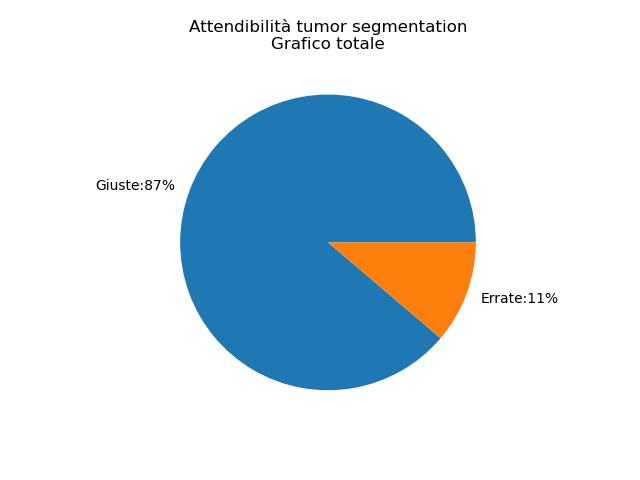
\includegraphics[width=8.5cm]{images/ts.png}
\end{wrapfigure}
Anche qui sono stati effettuati dei test per valutare la precisione della segmentazione su 200 immagini prese da una delle 4 directory del dataset formato matlab.
Per valutare se,data un immagine in input, il programma trova il tumore correttamente,sono state confrontate le seguenti immagini
\begin{itemize}
    \item Immagine nera con solo il tumore trovato dal programma
    \item Immagine nera con il tumore presente nel file .mat(cjdata.tumorMask)
\end{itemize}
La funzione per il confronto immagini ritorna un 'p' da 0 a 1 che indica quanto due immagini sono uguali(più 'p' è vicino ad 1 e più le immagini sono simili),per ogni p maggiore o uguale a 0.97 assumiamo che il tumore sia stato preso con esattezza,in tutti gli altri casi no.
Quindi vengono considerati sbagliati i casi in cui la segmentazione non è precisa o i casi in cui il tumore è presente ma il programma non lo trova.


\begin{conlusione}{Conlusione Segmentazione}
    E' possibile concludere che, con una certa approssimazione, la segmentazione del tumore ha una
    percentuale di accuratezza del 90 percento, per cercare di migliorare ancora di più andando
    ad alzare la percentuale è possibile provare a migliorare l'accuratezza dello skull stripping 
    e/o l'estrazione del colore medio, questo perchè influenzano la segmentazione in quanto il 
    programma di segmentazione prende in input questi dati.
\end{conlusione}

\section{Interfaccia grafica }
L'interfaccia grafica a sua volta è suddivisa in 
\begin{itemize}
    \item Brain Tumor Segmentation
    \item Segmentation Filters
\end{itemize}

\subsection{Brain Tumor Segmentation}
Eseguendo il file "run.sh" situato nella directory principale, si apre un interfaccia in cui l'utente ha la possibilità di caricare un immagine dal file system (formati accettati .mat/.jpg/.png).
L'immagine scelta,apparirà nello spazio riservato alle due immagini "Before and After", sotto la sezione "Before".
Successivamente,è possibile avviare la segmentazione selezionando l'apposito pulsante "Start Segmentation".
L'immagine con il tumore(qualora ci fosse) segmentato apparirà sulla destra,sotto la sezione "After".
Inoltre, viene mostrata l'area del tumore trovato e la probabilità che il programma abbia trovato effettivamente un tumore.
Se il programma non trova nessun tumore,a destra comparià la scritta "TUMOR NOT FOUND".
Infine,l'utente può salvare l'immagine del tumore segmentato, selezionando il pulsante "Save Output", scegliendo,all'interno del proprio computer,dove andarla a memorizzare.
\begin{figure}[H]
    \centering
    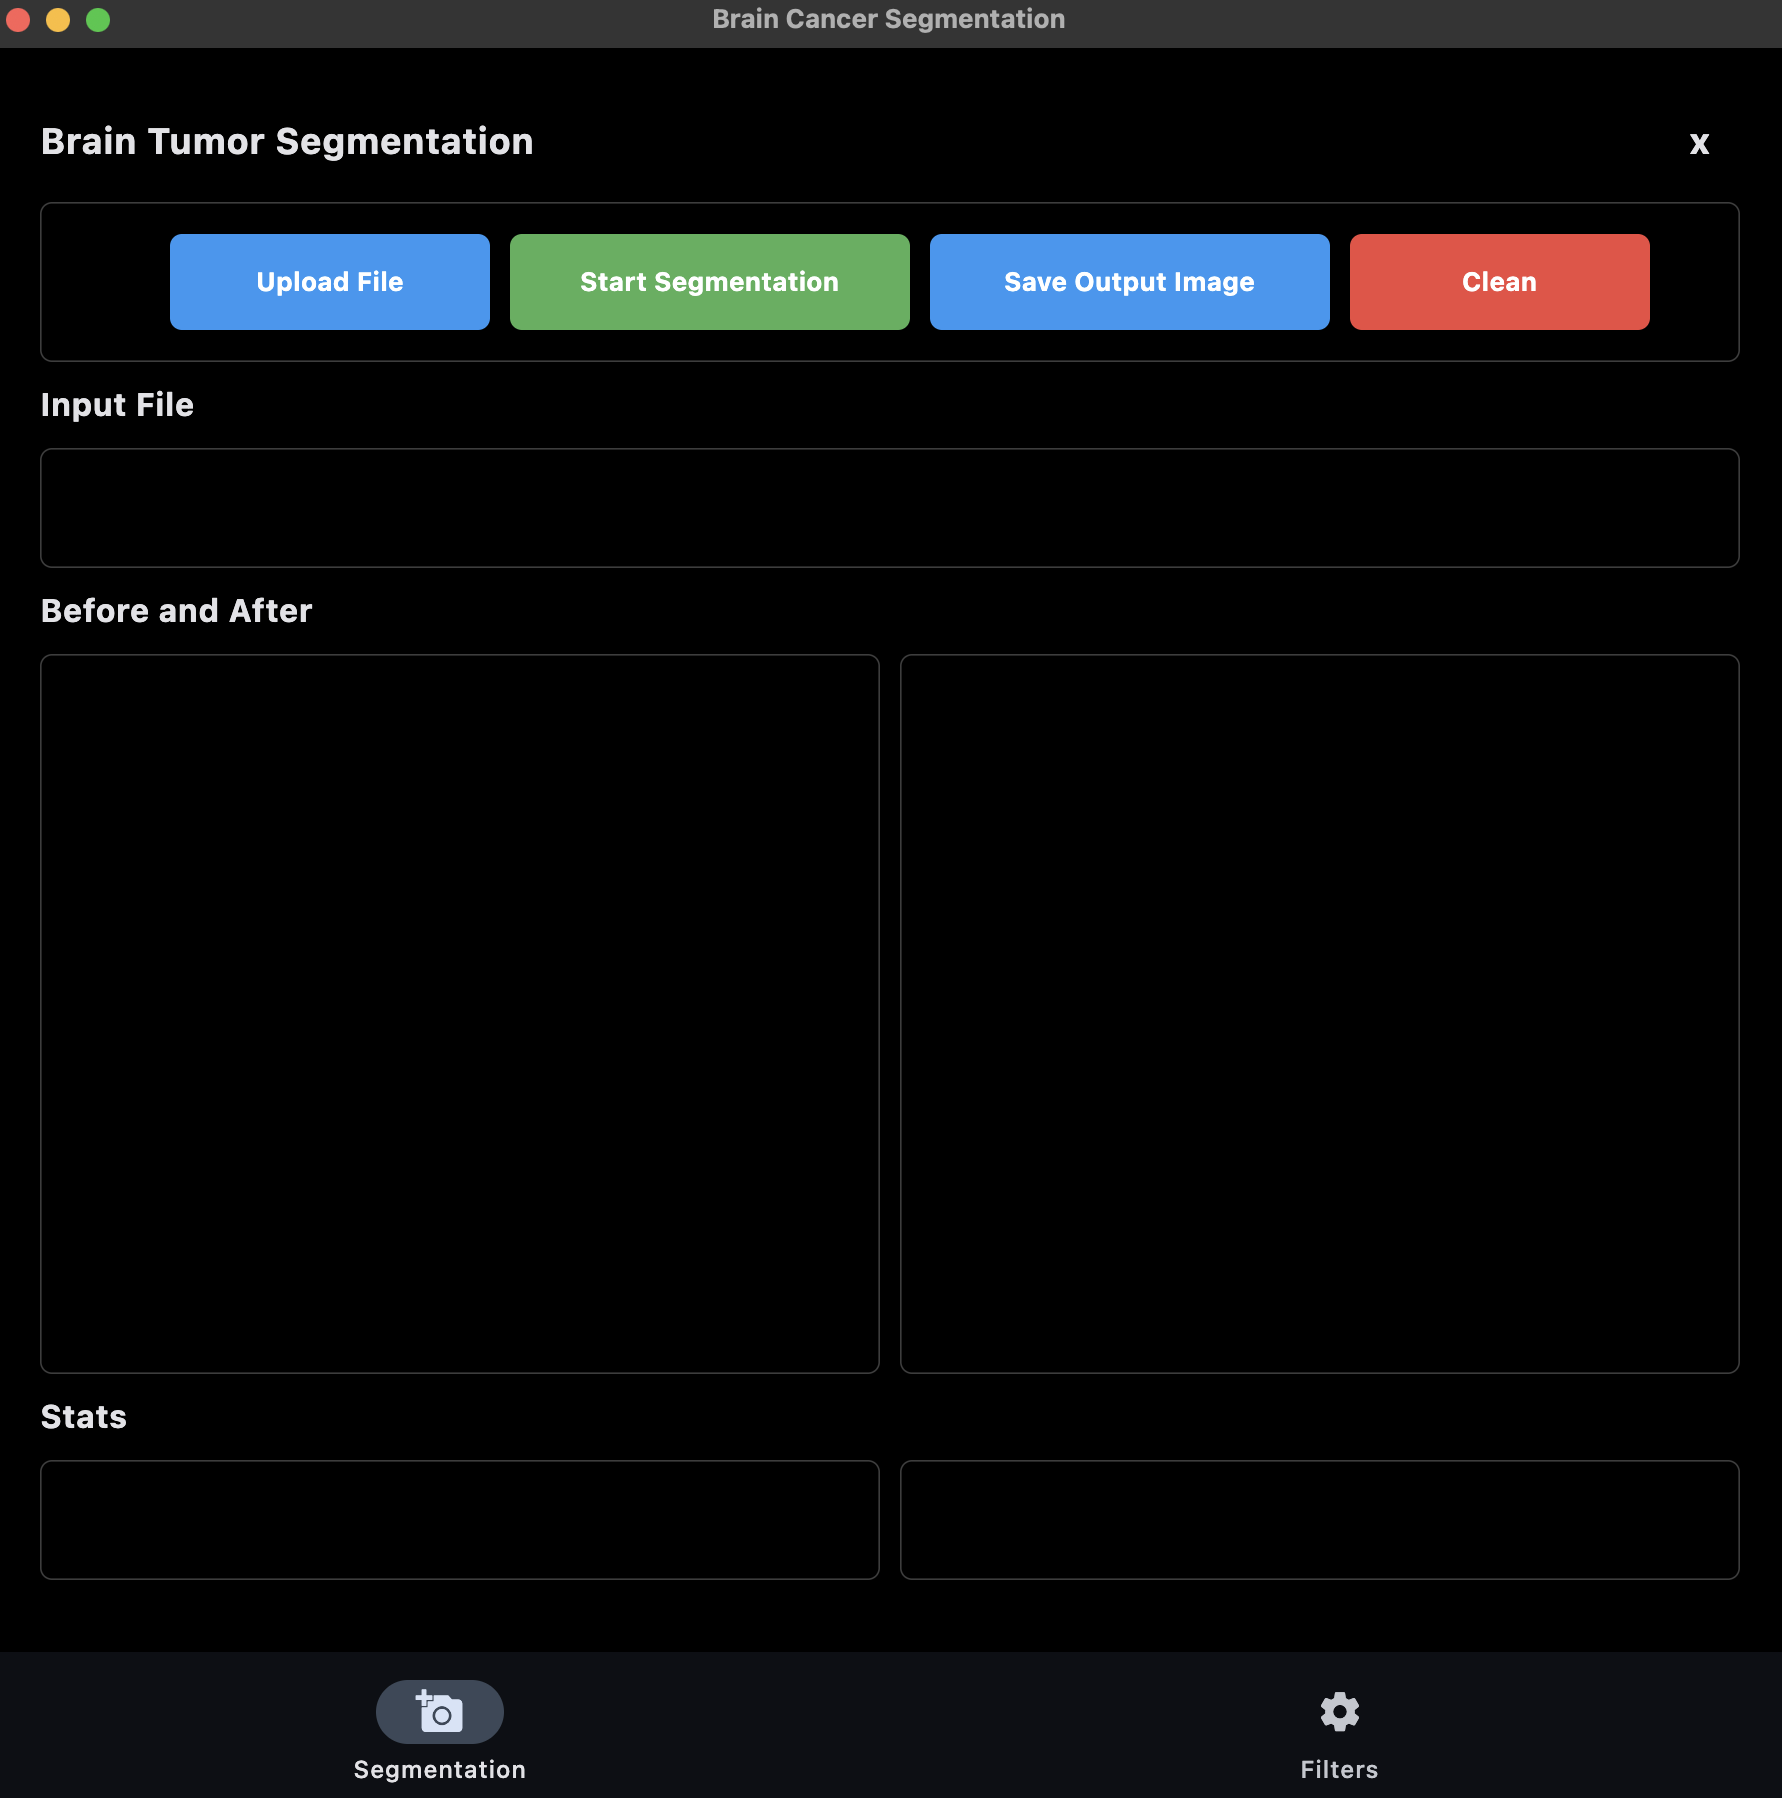
\includegraphics[width=7.5cm]{images/before.png}
    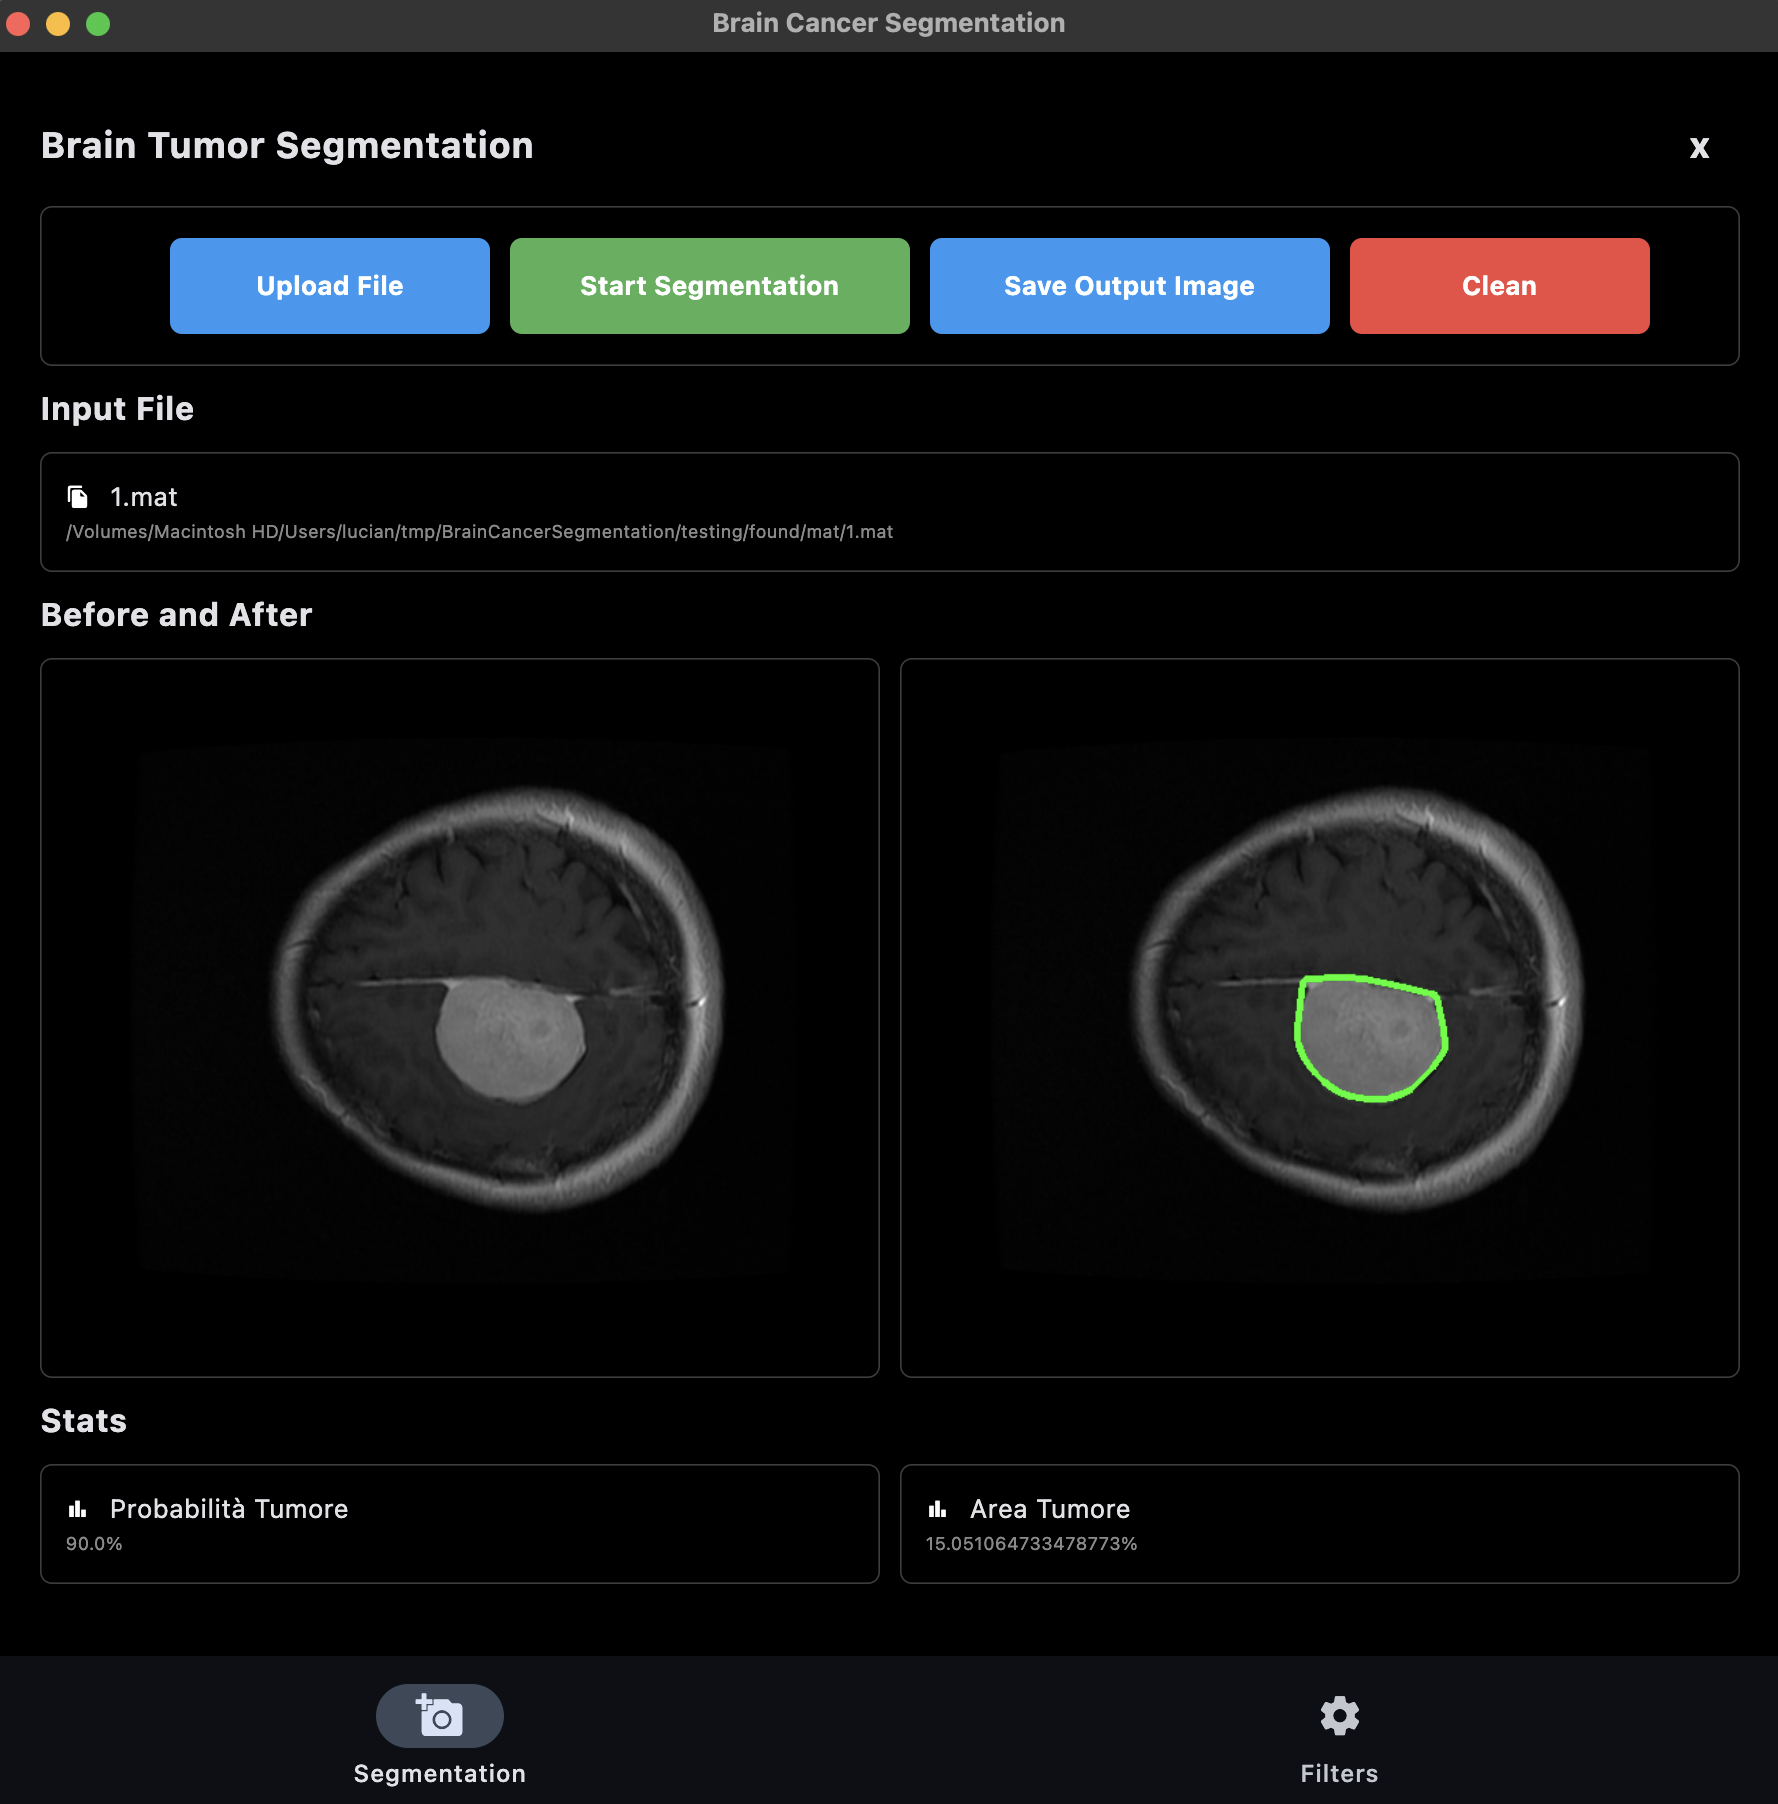
\includegraphics[width=7.5cm]{images/after.png}
\end{figure}

\subsection{Segmentation Filters}
L'utente può caricare un immagine che il programma ha generato in un primo momento,ovvero un immagine con il tumore segmentato e applicare dei filtri.
Ad esempio è possibile aumentare/diminuire il colore del tumore in modo da aumentare il contrasto con il resto della foto.
E' possibile vedere e salvare l'immagine contenente solo il tumore, su sfondo nero.
Infine,è possibile eliminare il segmento del tumore che il programma aveva creato,portando l'immagine come era prima della segmentazione.

\begin{figure}[H]
    \centering
    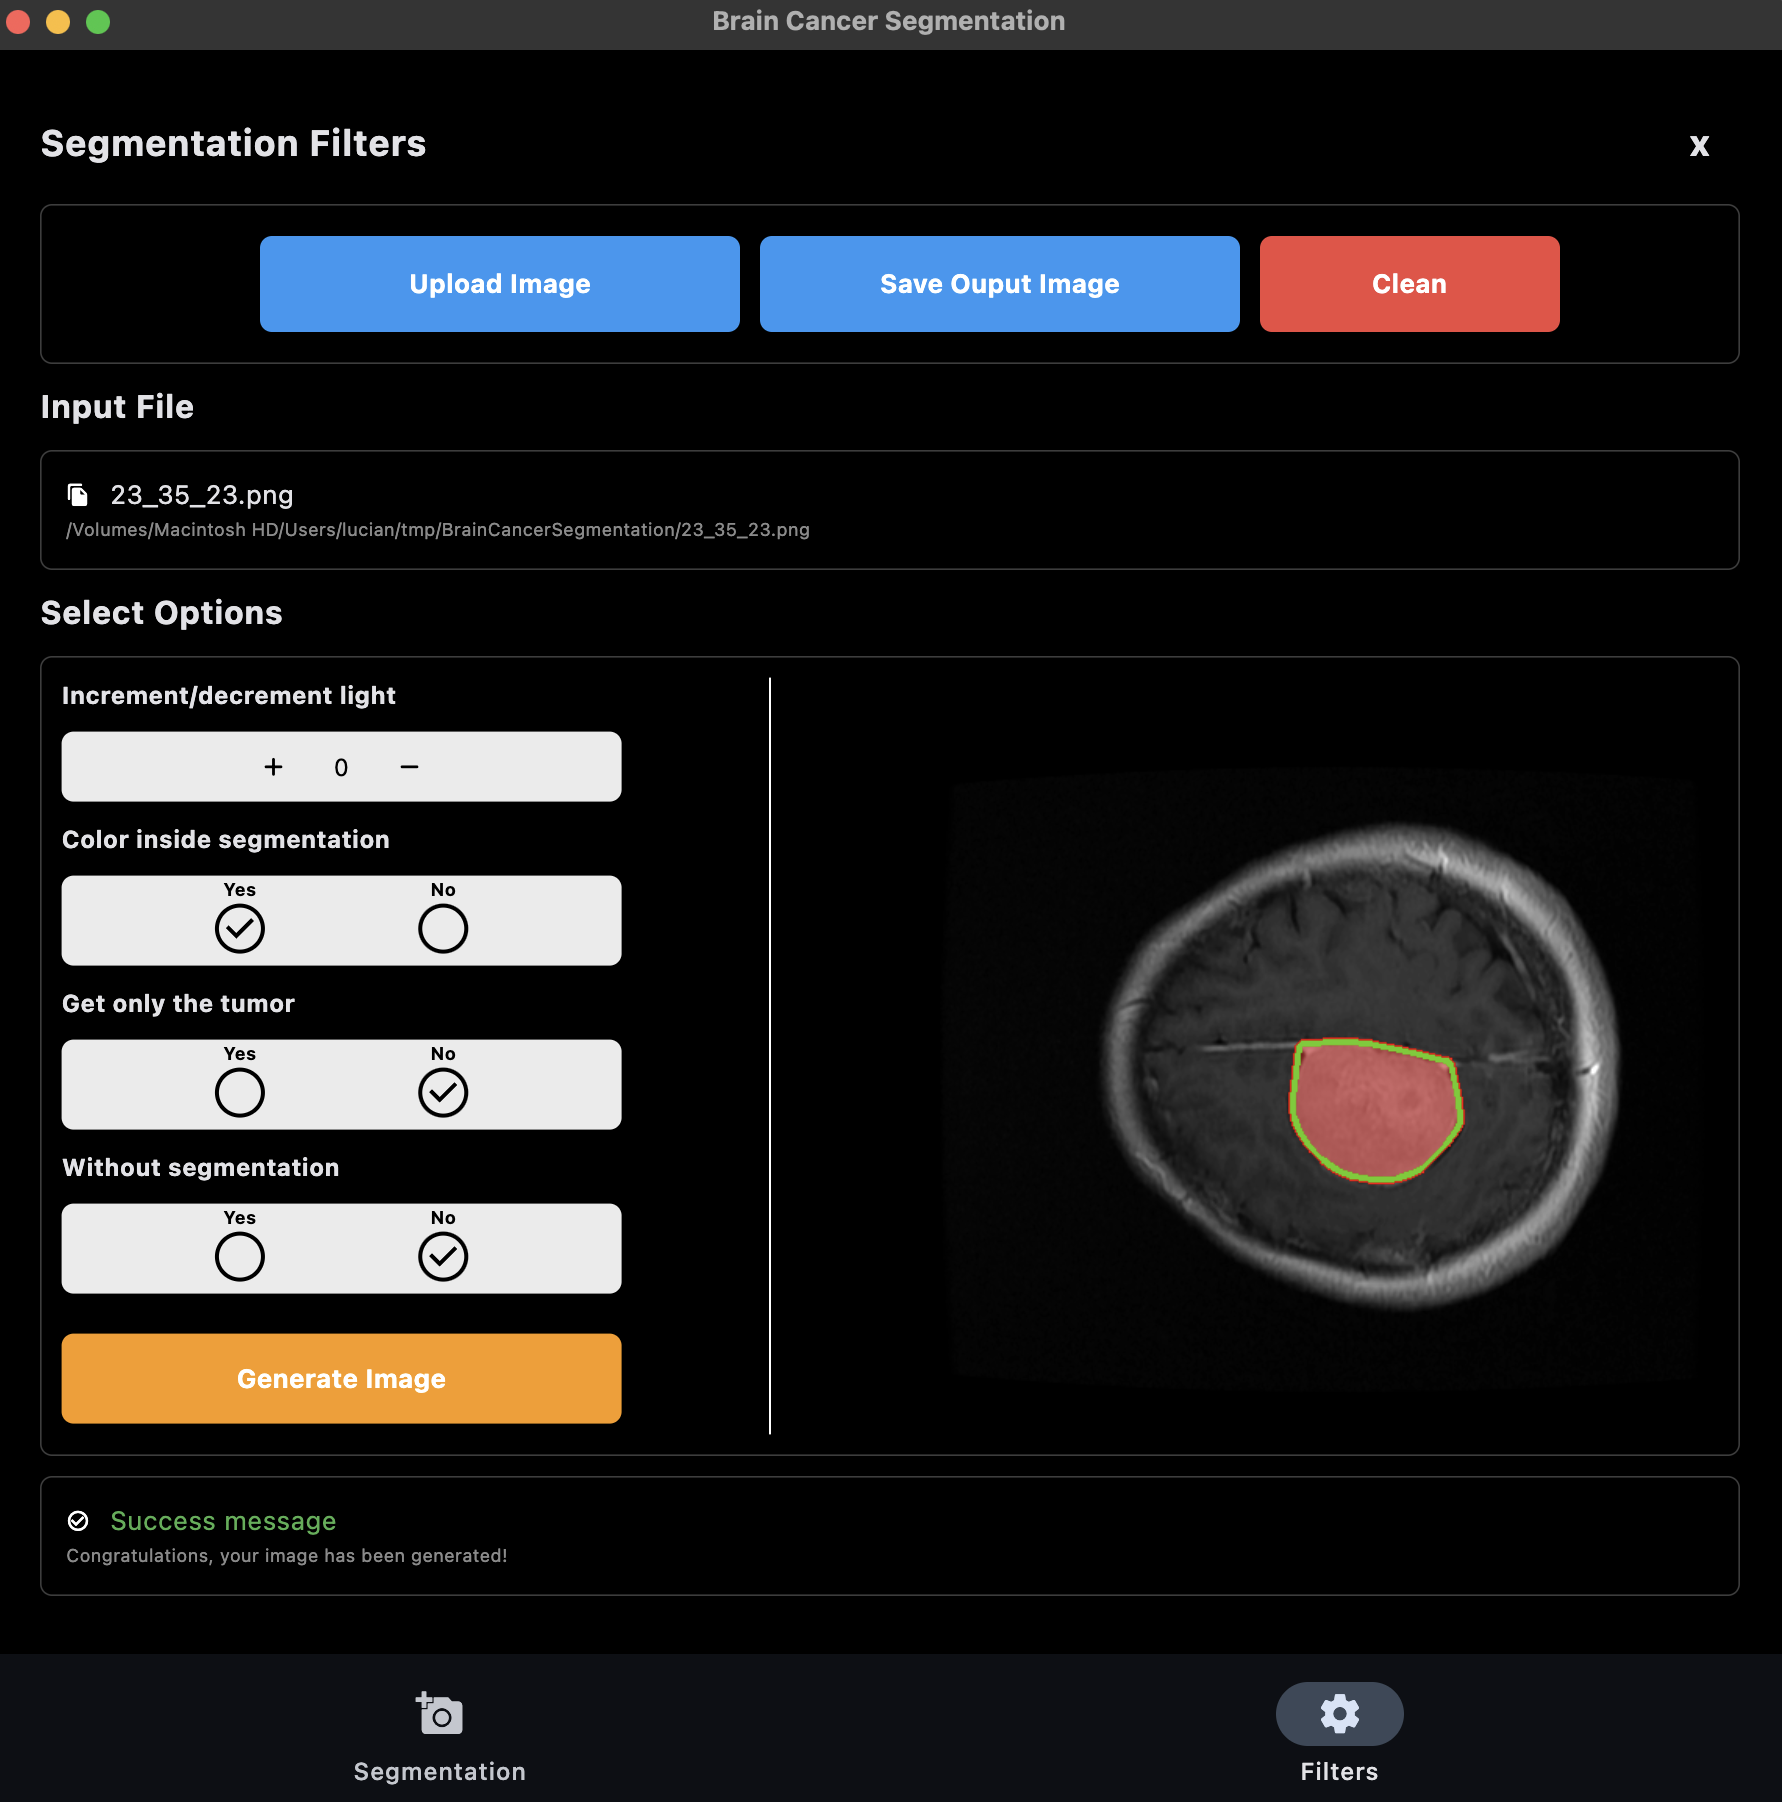
\includegraphics[width=7.5cm]{images/filters.png}
    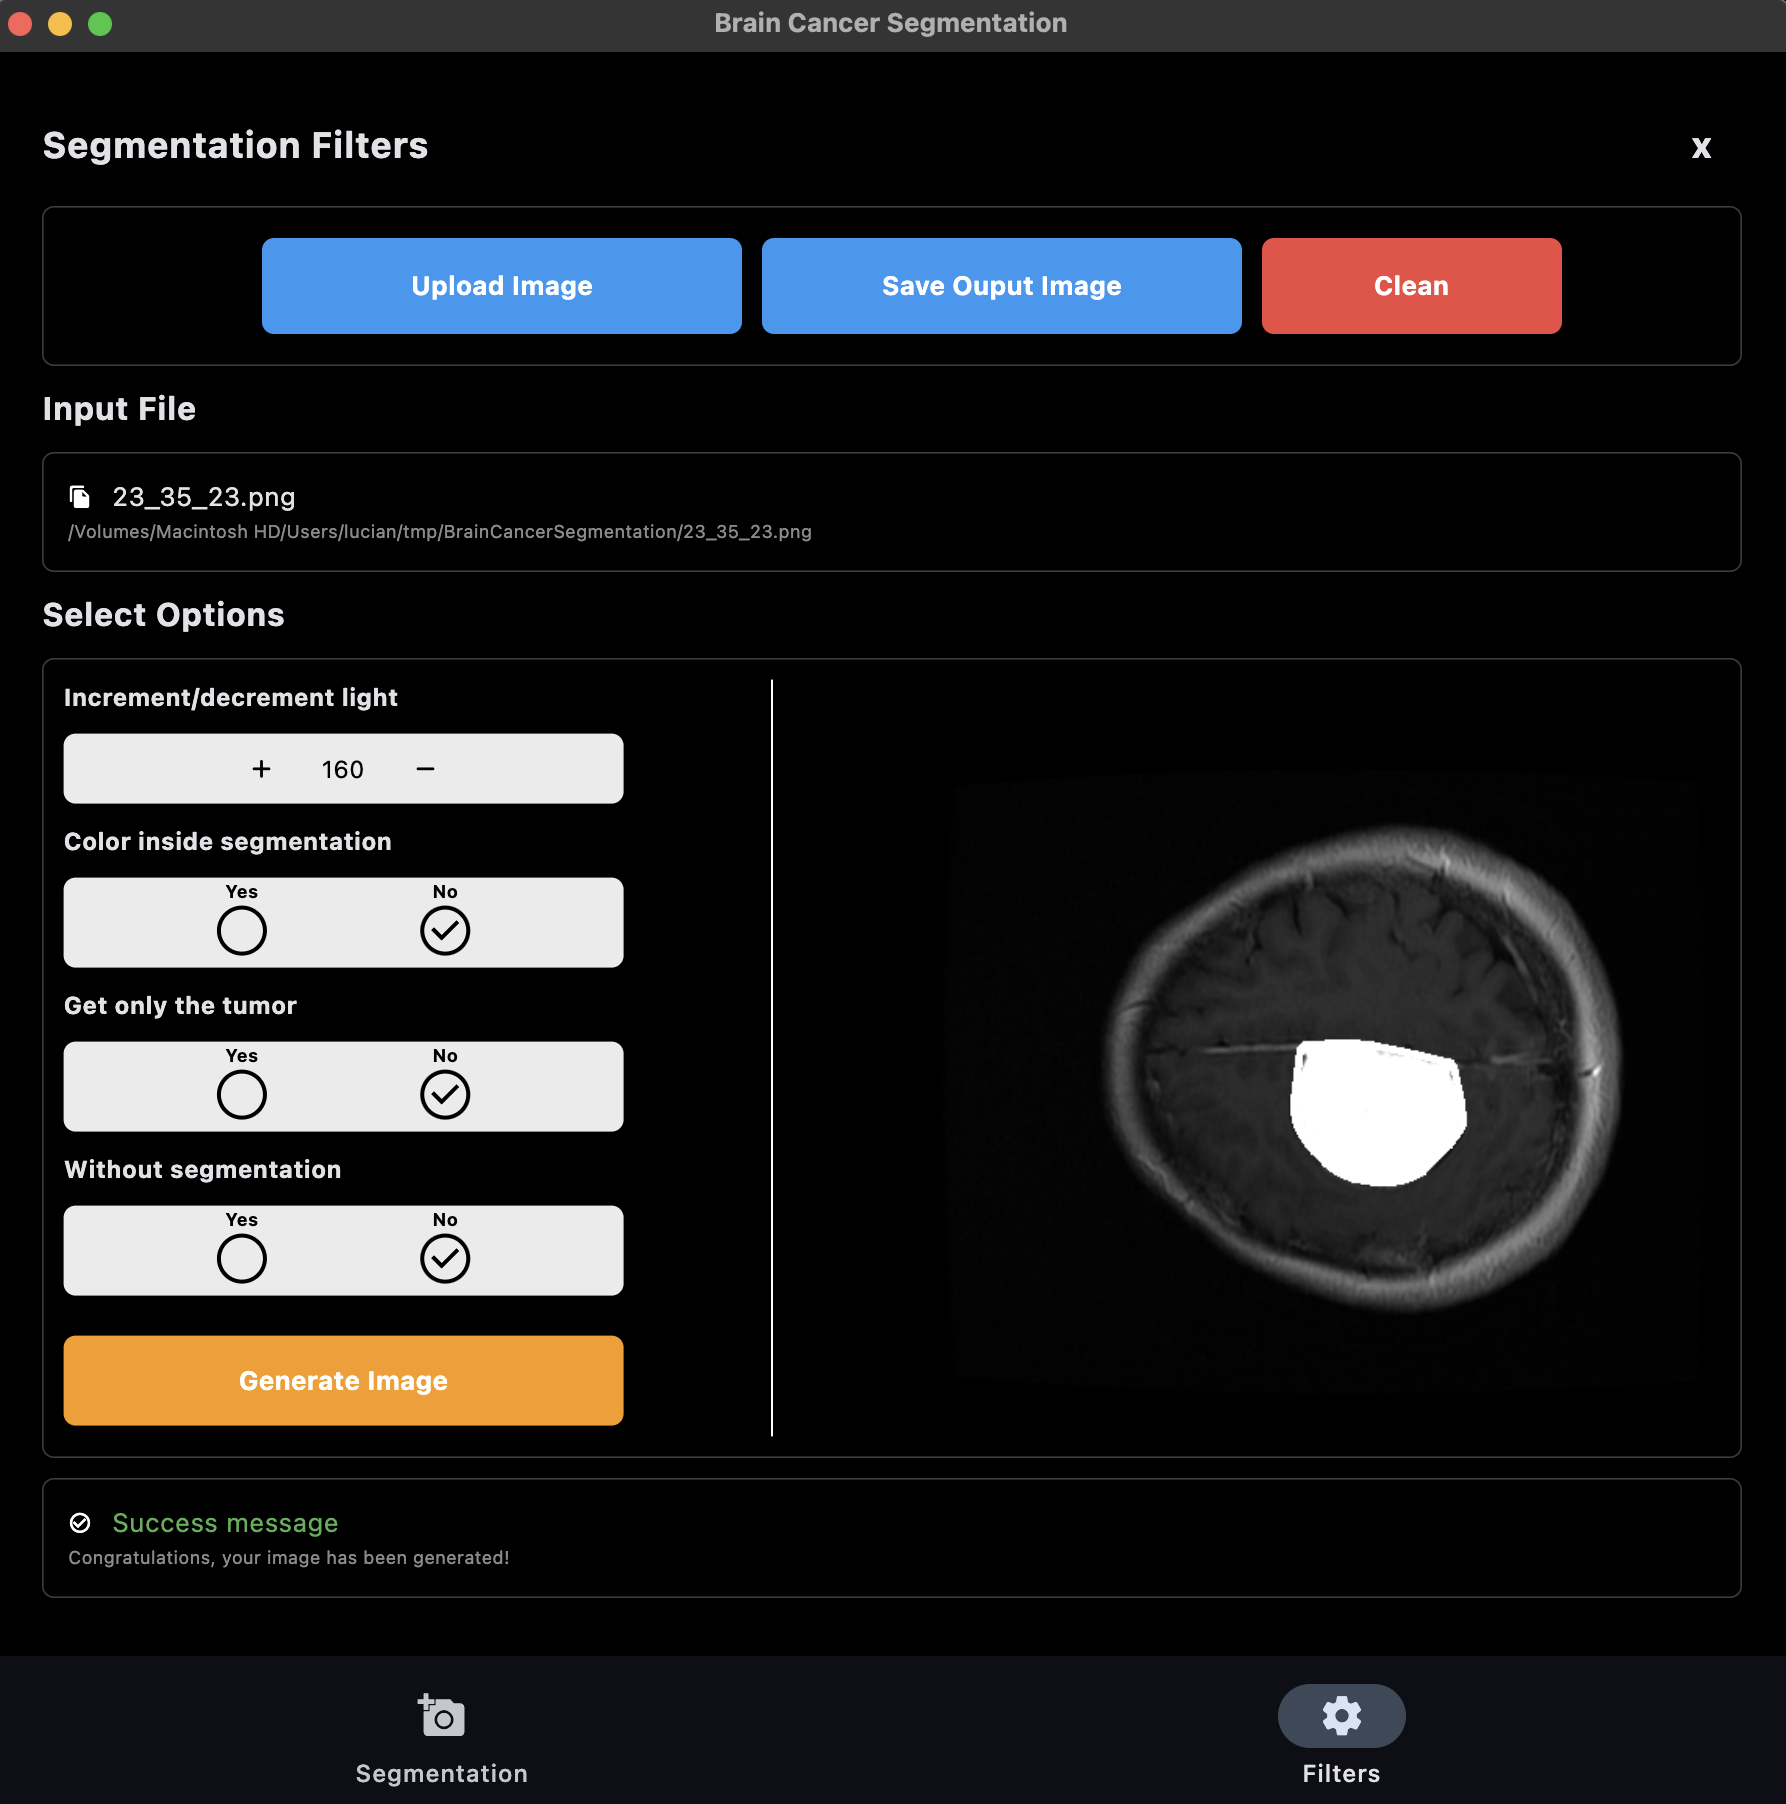
\includegraphics[width=7.5cm]{images/filters_2.png}
\end{figure}

\subsection{Esempio di esecuzione}
Illustriamo al seguente \href[]{https://youtu.be/7hxn5r4IMzw}{link} un esempio di esecuzione dell'applicazione.
\end{document}